\chapter{Ripple Attacks}
\label{ch:Chapter2}

\section{Motivating system: Artificial Pancreas System}

We use a DNN based \ac{APS}, closed-loop model, by Dutta et al. \cite{10.1007/978-3-319-99429-1_11}  as our motivating example for illustrating a \ac{RFDIA}. 
A patient relies on  the APS to correctly determine the next dose of insulin to be injected. \karthik{You should mention what's the time period.}

\begin{figure}
	\centering
	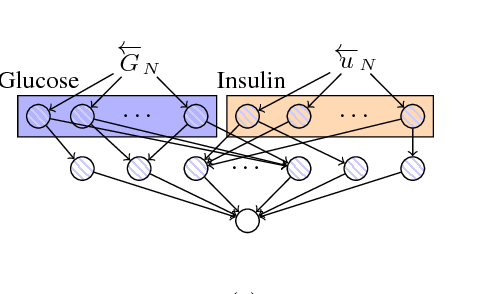
\includegraphics[width=0.7\linewidth, height=0.3\linewidth]{Images/APSDNN}
	\caption[APS DNN]{APS DNN designed by Dutta et. takes in 74 inputs of insulin and glucose. The next layers form connections between the insulin and the glucose to make predictions.[8]}
	\label{fig:apsdnn}
\end{figure}

%How is APS constructed?
The APS architecture is explained in Section 2.4. 
We examine the \ac{APS} controller model from Dutta et al., which has a feed-forward architecture. 
The DNN for APS creates mappings between the insulin and the glucose values that allow for the prediction of future insulin values as shown in Figure 3.1. 
The insulin and the glucose values are the values collected from the sensors and the actuators. 
The model has 74 inputs in total, where 32 inputs are the glucose, and the other 32  are insulin values collected every 5 minutes.
 The DNN layers use these values as inputs to predict the next value. 
 This implies that the future value is predicted based on the inputs from the previous set of values. 


%Defense mechanisms
There are two phases in a \ac{DNN}s life \karthik{too informal}; training phase and inference phase. 
During the training phase, there are three \ac{DNN}s that are trained in an \ac{APS} to predict the next outcome. 
This is done to design defense mechanisms such that the patient is not overdosed with insulin \karthik{I removed the in presence of bugs}.  
The two \ac{DNN}s are separate from its main decision making controller. \karthik{Which two DNNs?}
These \ac{DNN}s are trained based on the latest 30-day patient data to understand the standard injections for a patient over time. \karthik{So how do you get this data?}

One \ac{DNN} learns a lower threshold on injection amount; the other learns an upper bound on injection amount. 
Hence, for every time of the day based on the previous patient characteristic, the minimum and the maximum values are known. 
However, the system will not detect  an adversary  who manages to always administer the maximum allowed dosage. \karthik{How ? Via ripple attacks ?}  
Hence, the attacker needs to identify inputs and  perturb them  such that the output changes the maximum  allowed dosage for every injection, \karthik{Why maximum ?}
  while being lower than the upper threshold to avoid detection. 


\section{Attack Model}
The attacker's goal is to manipulate the sensor measurements to conduct FDIAs without triggering alarms as shown in Figure 3.2. 
The attacker can use network noise or physical means of sensor tampering to attack the systems. \karthik{Citation}
 
\begin{figure}
	\centering
	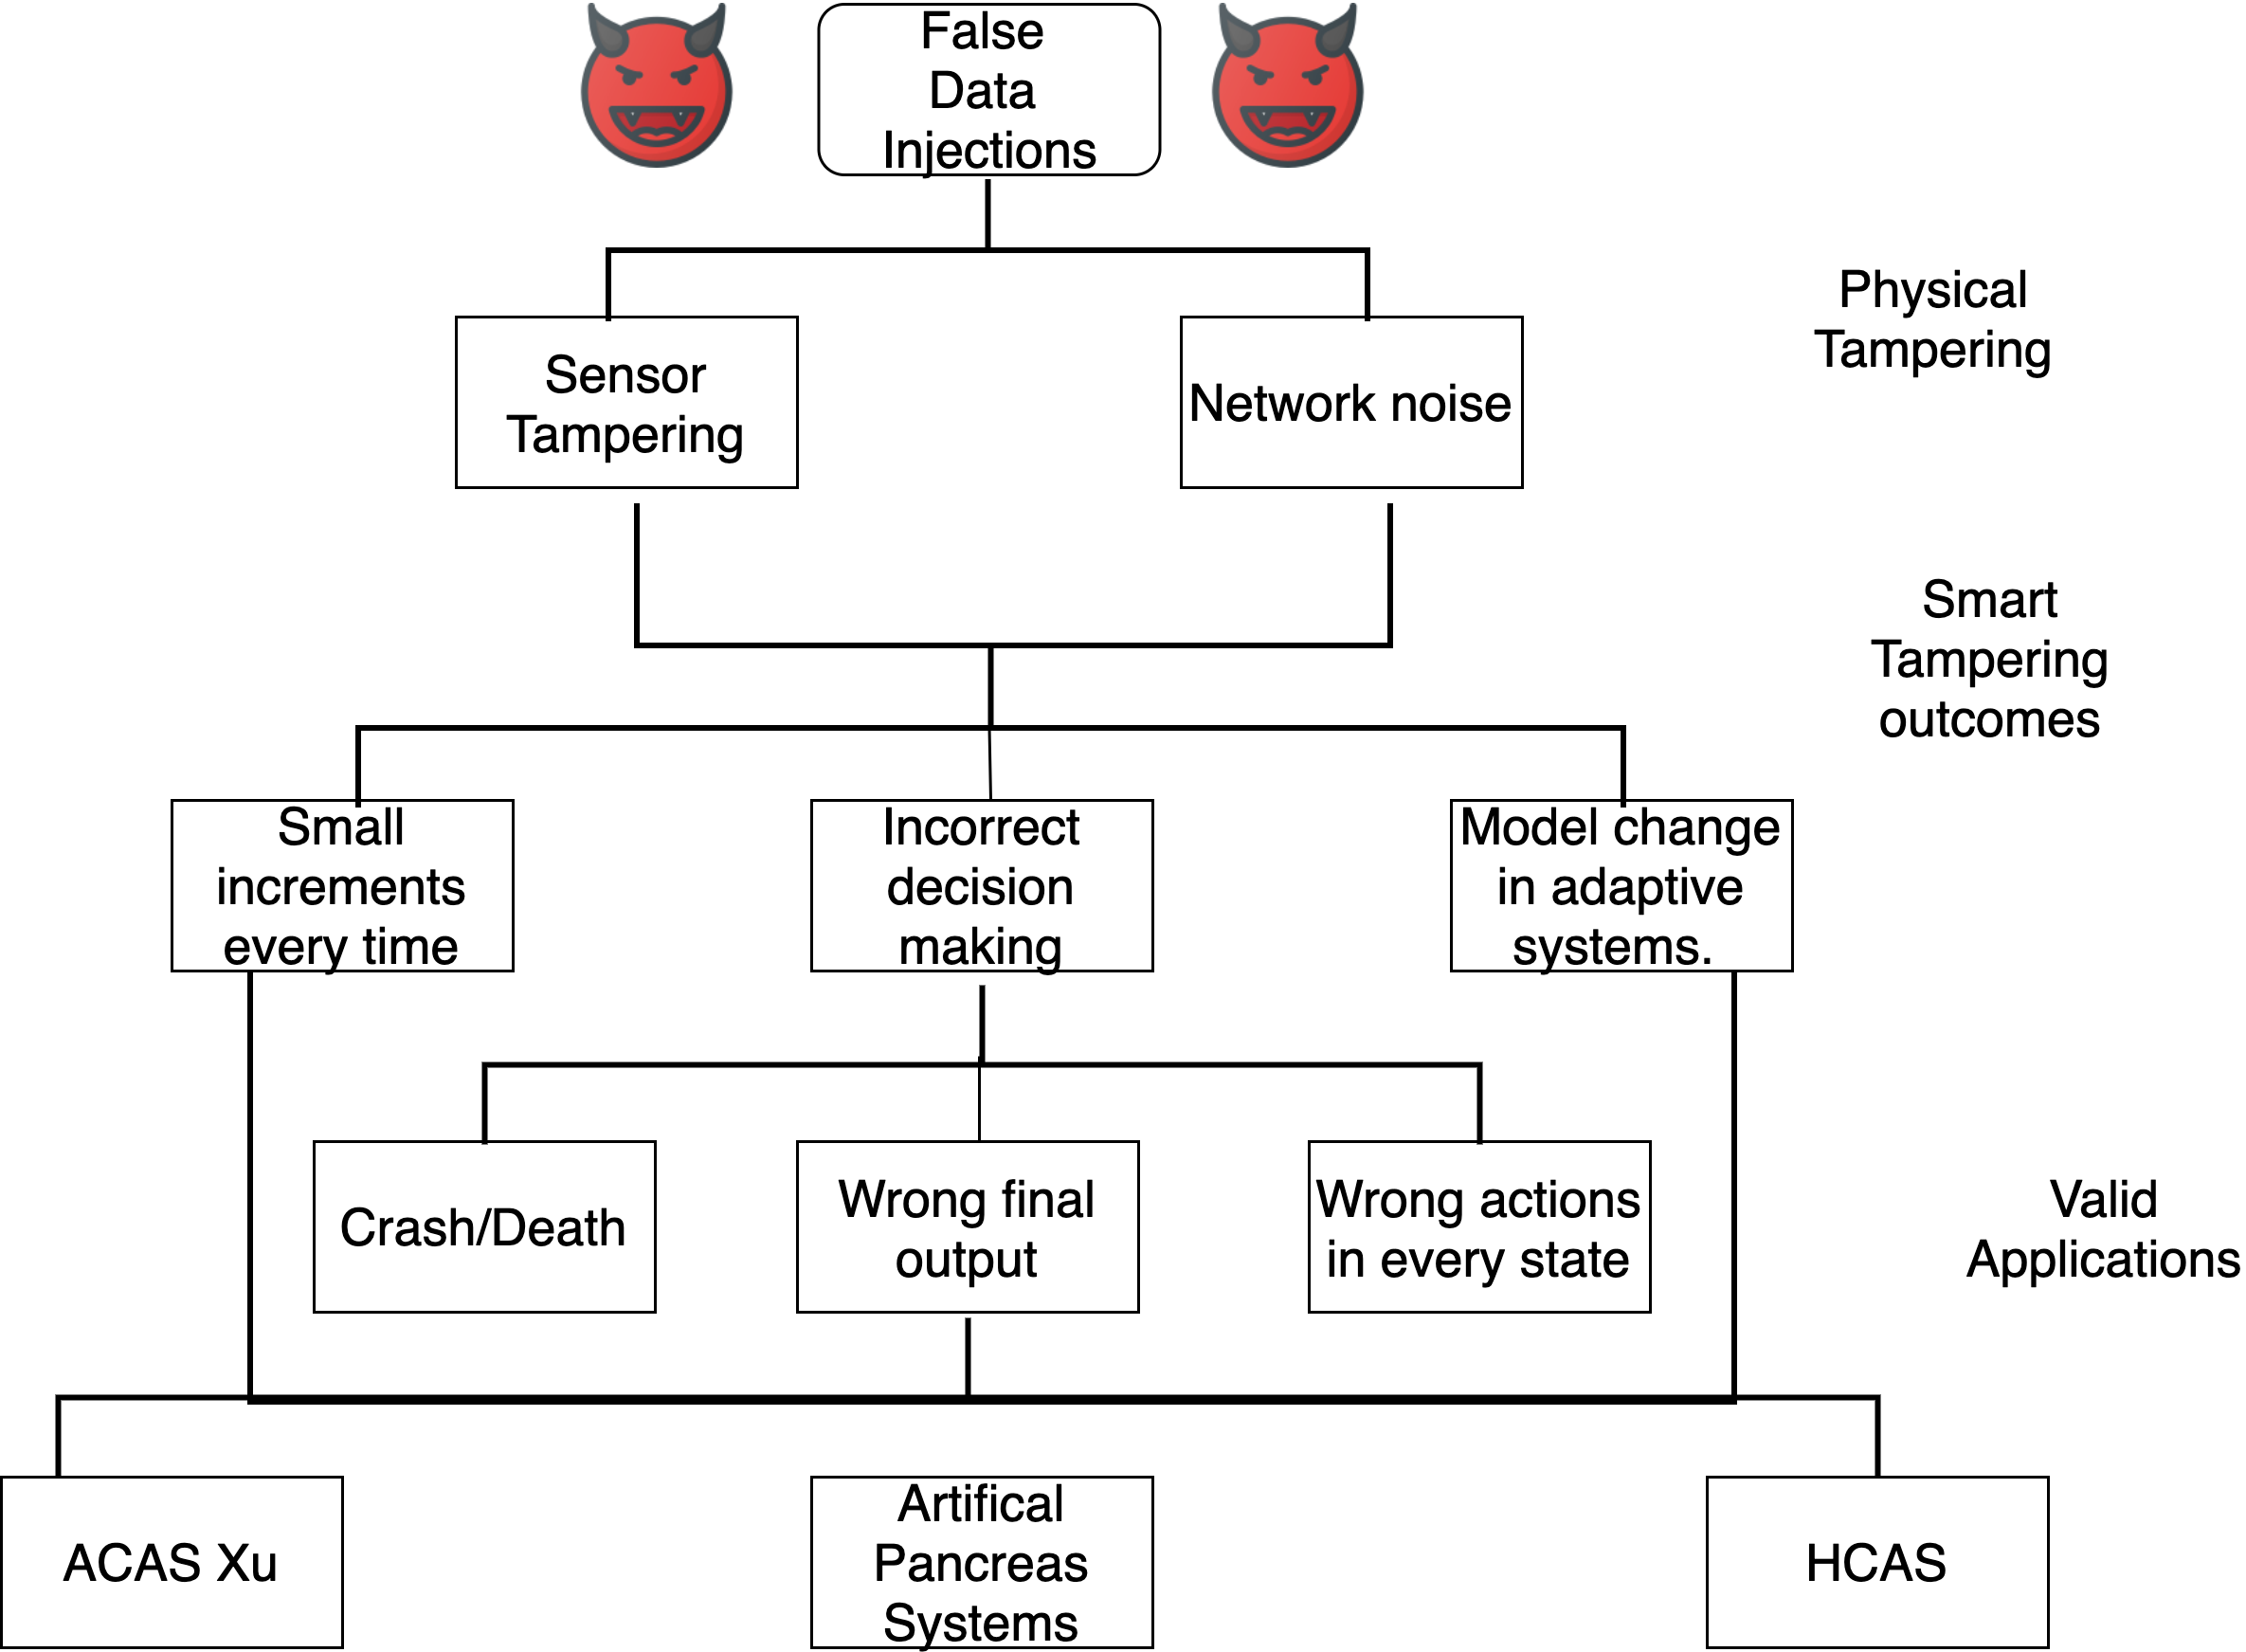
\includegraphics[width=0.7\linewidth]{Images/Attackmodelphysical}
	\caption{Attack model}
	\label{fig:attackmodelphysical}
\end{figure}

We assume that the attacker has following capabilities:
\begin{enumerate}
	\item The \ac{DNN}  architecture  is known to the attacker for e.g., a feed forward  network in case of an \ac{APS}. This information easy to find, as the architectures are  usually public information for the systems. 
	\item  The weights and bias of the \ac{DNN}  architecture through a read-only access to the system.  
	\item The attacker cannot modify the code but only the inputs to the model.
	\item The \ac{DNN} contains ReLU as its activation function. \karthik{and no other function.}
	All three systems in this work contain ReLU.
\end{enumerate}

\subsection{Strawman attacker}
The first way to attack the system would be to change all the 74 values that are the inputs to the DNN.
 If all the inputs are changed, the final output prediction is going to be wrong. The problem in this particular scenario is that 
 these inputs are collected every five minutes from the sensors attached to the patient. 
 This means that the attacker will have to conduct FDIAs every five minutes when the data is being collected to cause a change in the output.
 We demonstrate these attacks in Chapter 6 and they are quite easy to conduct. \karthik{I'm not sure why we say this}  
  Doing this is not feasible\karthik{Too strong} in a practical scenario and hence, the attacker needs a better way of attacking the system. 

\subsection{Sophisticated Attacker}
A more sophisticated approach to attack the system would be by perturbing one or two inputs out of the 74 inputs that cause a change in the output. There are two ways to proceed when the attacker tries to change just one or two inputs at a time. 

\subsubsection{Attack 1}
The attacker can randomly choose two inputs and perturb them by huge amounts. 
This will indeed cause a wrong output prediction. 
However, if the input is perturbed by large amount, the error detection mechanisms will recognize that there is an anomaly. 
To prevent this the attacker can choose to perturb the two inputs by small amounts. 
However, perturbing any two random inputs by very small amounts might not necessarily lead to a wrong output prediction (Chapter 6). \karthik{Use chapter references, rather than hardcode them - we may move these around.} 

\subsubsection{Attack 2}
Adding one more layer of sophistication, the attacker supposedly\karthik{They either know or they don't, not supposedly} 
knows the critical inputs or the input whose perturbation can lead to wrong predictions. This will be a more targeted approach for attacking the system since the input selection will not be random. 
However, not knowing the precise amounts by which the critical inputs should be perturbed can lead to an unsuccessful attack. 
If the perturbation is too high, it will trigger the error-detection mechanisms, 
and if it is too low, it will not affect the output (Chapter 6). \karthik{Reference hardcoded}

\subsubsection{Attack 3}
The most sophisticated means for an attacker to attack the system would be to know precisely which inputs to perturb and by what amounts,
 such that the output prediction is wrong. 
To do so, the attacker needs an advanced technique that in limited time, finds the critical inputs (as we call them\karthik{Refer to Chap 2 - problem formulation}),
 and also the small perturbations that can ensure a wrong output prediction. 

\karthik{I recommend merging this with the next chapter as it's too small otherwise}

%Our motivation for designing the technique were these different ways of attacking the system that can automatically synthesize attacks in an efficient way. 













